\chapter{PCB 布线攻坚：从 146 到 0}
\label{ch:pcb}

布局定稿时，四层板上还留着 \textbf{146} 个未连接；Gerber 交付时，这个数字是 \textbf{0}。本章按时间线复盘这条下降曲线——146$\to$17$\to$6$\to$0——的四个阶段：自动布线器的两轮冲锋、一次靠目视检查才抓到的隐形事故、两个几何模型的修正，以及自研工具链的收官。每一阶段对应一次 git 提交，数字与细节均可回溯。

\section{布局定局与层叠}
\label{sec:pcb-layout}

骨架定稿（commit \texttt{41e697e}）：90$\times$75\,mm 四层板，层叠为 L1 信号+元件 / L2 GND 整片 / L3 电源分区（5V+3.3V）/ L4 信号；电源过孔 54 个、GND 缝合过孔 36 个。板尺寸从 80$\times$70 放宽到 90$\times$75 是布局实践的结论：8 个螺丝端子单排就需要 $\ge$88\,mm，17 个连接器在原尺寸下已经饱和（修正 \#13）。布局收敛后，自动布线器（自研 A* 双层版）已建立但尚不完善，剩余 146 个未连接决定交给 Freerouting 与后续攻坚。

\section{146$\to$17：freerouting 双轮与布线后清理}
\label{sec:pcb-freerouting}

commit \texttt{c3337a3}：采用 freerouting v2.4.1（headless CLI，DSN 导出、SES 回灌）跑两轮 rip-up\&reroute 与 BatchOptimizer，未连接从 146 降到 17，短路为零。布线后的清理同样关键：重建电源平面（GND 全实连）、把 0.25\,mm 线宽回退到 0.2\,mm 消除约 130 处间距违规、\texttt{zones\_intersect} 与 \texttt{starved\_thermal} 清零。

\section{天线禁布区事件：目视检查抓到的隐形事故}
\label{sec:pcb-keepout}

这一阶段最有教学价值的不是布通率，而是一次\textbf{目视检查}的战果。用户强制要求对顶/底面 2400$\times$2000 渲染图逐区人工检查，配合程序化核实，结果发现：布线脚本 \texttt{route\_pcb.py} 在重建电源平面时，\textbf{把 ESP32 模组天线下方的禁布区删掉了}——GND 与 +3V3 填充直接铺进了天线正下方（\texttt{HitTestFilledArea} 四层命中）。这类事故不会报任何 DRC 错误：铜皮完全合法，只是 WiFi 从此没有辐射窗口。修复是补写 \texttt{fix\_keepout.py}：重新写入 \texttt{ANT\_KEEPOUT} 规则区域（$x\,19.5$--$36.5$ / $y\,0.2$--$6.4$\,mm，四个铜层禁填充/走线/过孔），重灌后 6 个探测点零命中，DRC 无新增。安装孔四处全净空、走线无乱麻。教训只有一句话：\textbf{自动化的每一步"重建"，都可能静默丢弃它不认识的约束}——这就是本书坚持"渲染图逐区目检+程序化复核"双轨的原因。

\section{模型与工具攻坚：17$\to$6}
\label{sec:pcb-tooling}

接下来是三个提交的连续攻坚。第一步修模型（commit \texttt{d549f4a}）：GND 过孔避让 C1.1 时发现旧的碰撞模型假设"矩形焊盘四角伸出孔半径一半之外按圆近似"，几何上不成立——改为点对旋转矩形的精确距离计算，孔距规则随之从 3 收紧到 2。第二步修布局（commit \texttt{cd47167}）：删坏线、补 5V 过孔、重连 D10.1；把 HD 从 (77,62) 移到 (68,65) 给 D10 让出走线走廊，孔类违规 6$\to$1、悬空过孔 2$\to$1。第三步上自研工具链（commit \texttt{a38172a}）：\texttt{boardgeom} 提供全障碍感知的落点库（焊盘含孔、走线、过孔、NPTH、板边、禁布区），\texttt{netdoctor} 做填充岛探测（PIP）、岛间跳线、焊盘逃逸与 In1--In2--B.Cu 多层 BFS 路由；配合 freerouting 三轮，未连接 17$\to$6，其余 error 类全零。遗留的 6 个未连接（R13/R29/C3--U3.2 口袋簇与 GND/3V3 zone 对）原本预计留给 GUI 手工收尾。

\section{6$\to$0：KRT 平面修复与终版打样包}
\label{sec:pcb-final}

收官来自 commit \texttt{d0eb1b2}：KRT \texttt{repair\_planes} 做全层修复——GND 三层平面与 3V3（12 区 11 路）、5V（6 区 5 路）的 In2 断区全部接通，\texttt{oracle\_reconnect} 连带解决了 R13/R29/C3--U3.2 口袋簇，未连接 6$\to$0，error 类全零，超出预期。工艺侧同步对齐：\texttt{min\_hole\_clearance} 25$\to$20（JLC 经济档合规），8 处 via-in-pad 标注需 IPC-4761 Type VII 填孔电镀。终版打样包（commit \texttt{fa2f138}）经三重验证交付：KiCad DRC、KRT \texttt{check\_connected}（75 网全通、refill 交叉核对）、禁布区探测零命中；顶/底渲染目视复查中发现的视觉疑点，经程序化裁决确认为 GND 填充纹理的误读。剩余的 111 条 DRC 记录全部是外观类（\texttt{silk\_over\_copper} 54、\texttt{courtyards\_overlap} 44 等），已列入豁免清单，嘉立创可制。

成品渲染如图~\ref{fig:pcb-top}（顶面：模组、端子排与天线净空区）与图~\ref{fig:pcb-bot}（底面：慢信号与 GND 缝合）。

\begin{figure}[htbp]
  \centering
  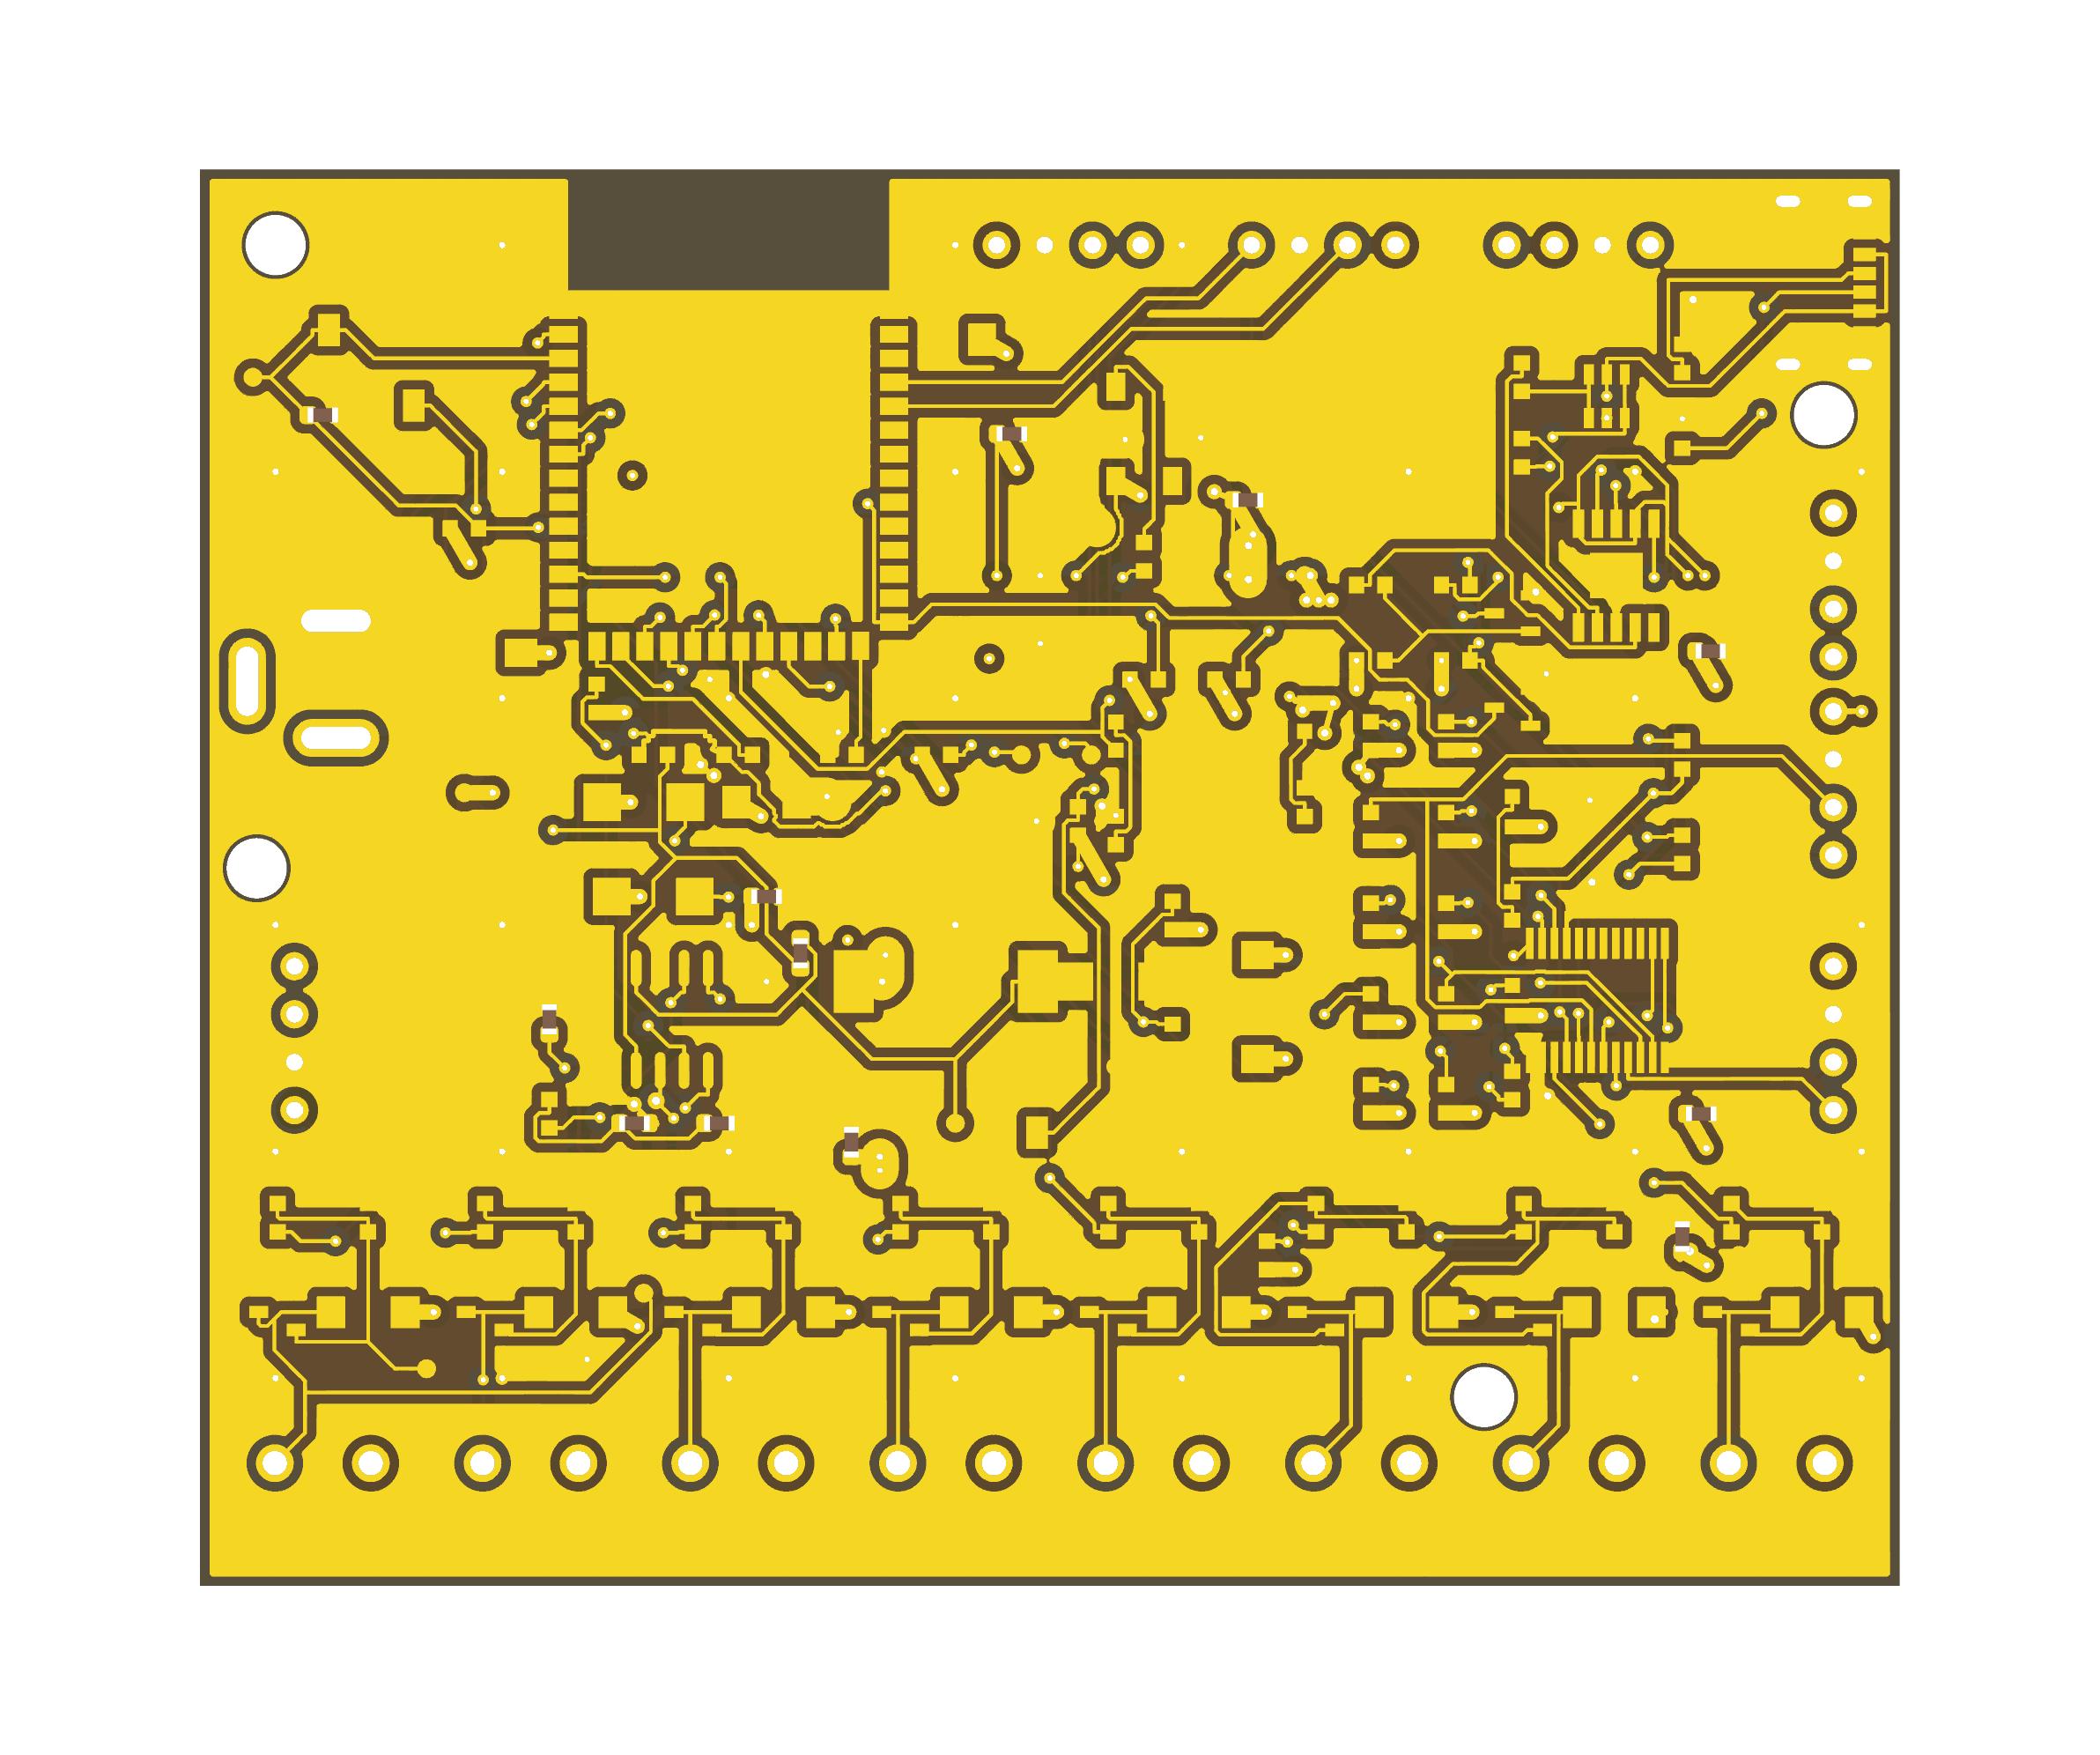
\includegraphics[width=0.92\textwidth]{figures/r_top.png}
  \caption{P1 顶面渲染：ESP32-S3 模组天线端朝板边，端子排单列布局}\label{fig:pcb-top}
\end{figure}

\begin{figure}[htbp]
  \centering
  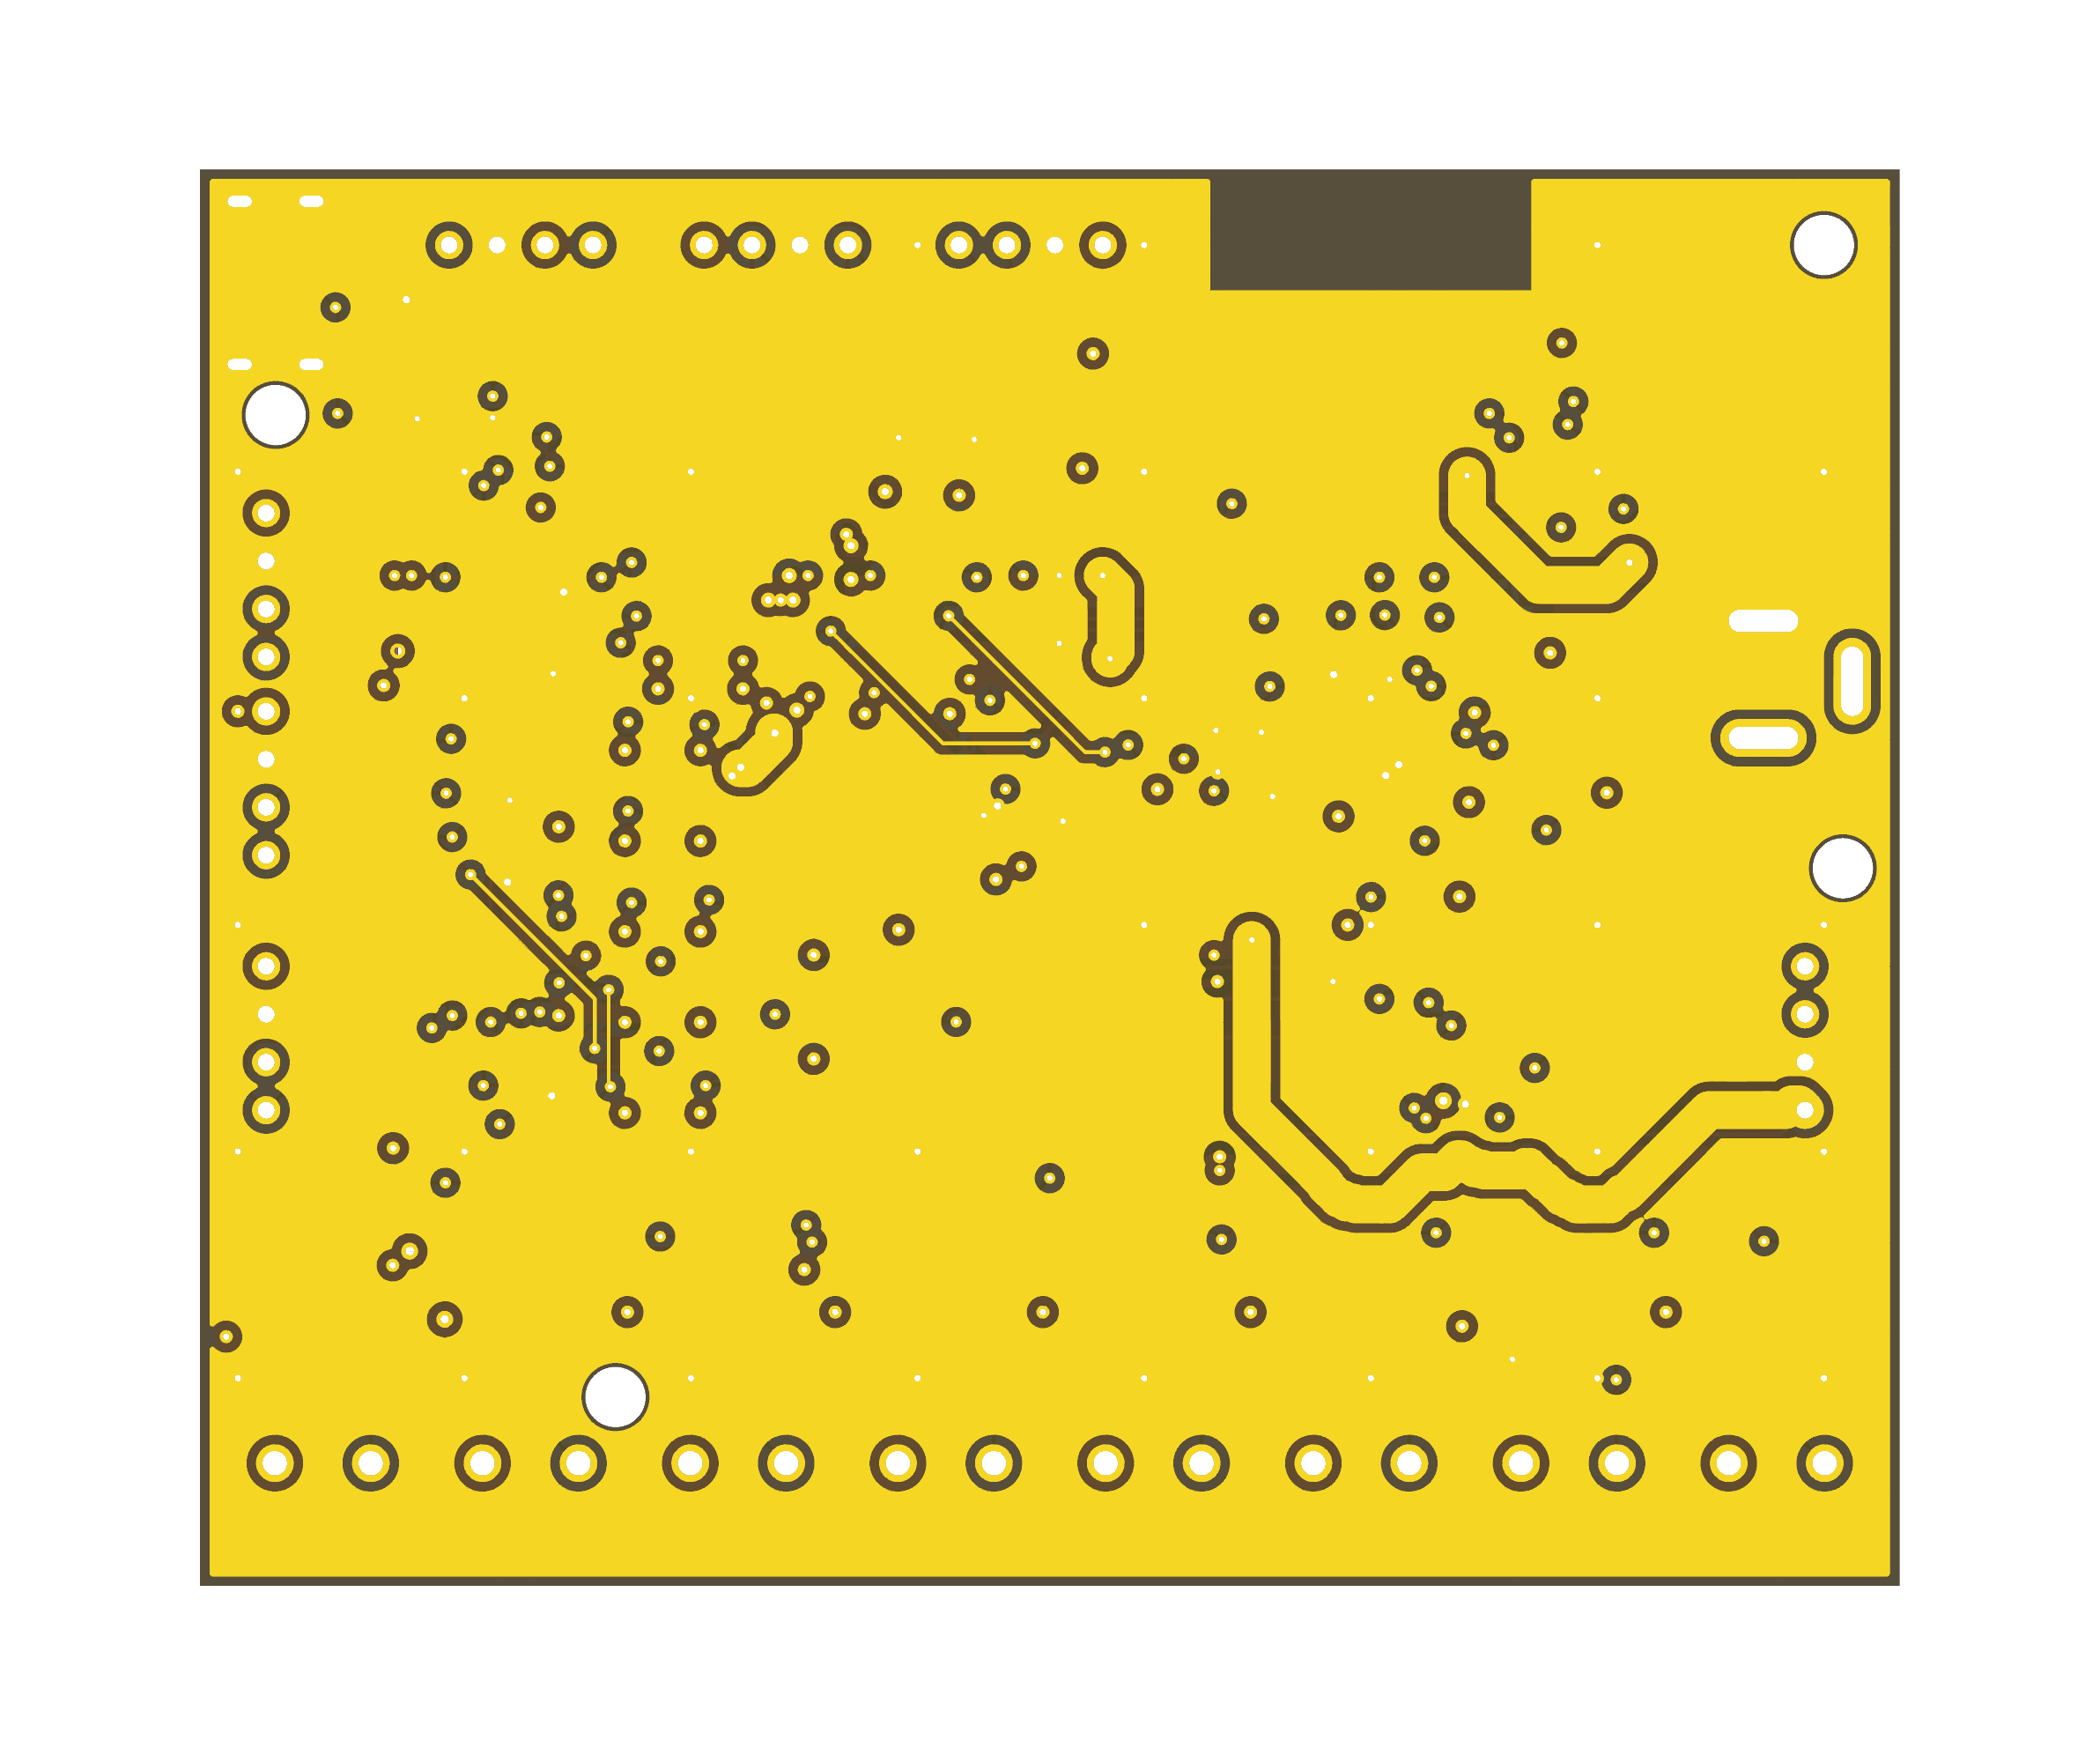
\includegraphics[width=0.92\textwidth]{figures/r_bot.png}
  \caption{P1 底面渲染：L4 慢信号层与 GND 缝合过孔}\label{fig:pcb-bot}
\end{figure}
